\chapter{Empirical Study of a Social Navigation Prototype}
\label{chapter:empirical}

This chapter details an empirical study of the prototype implementation we
developed in \chapterref{implementation}. First we'll frame what we think this
study should answer trough research problems and hypotheses. Then we'll go on
to describe the method we used for conducting this study before the results of
the study are presented. Based on the results we'll discuss our findings
before we close this chapter with some words about the limitations of this
particular empirical study.

\section{Research Problem and Hyoptheses}

\begin{quote}
  Can social navigation trough activity streams influence
  usage of an established web site?
\end{quote}

This question deals with how a specific social navigation technique, activity
streams, could potentially influence experiment participants' usage of a web
site.
From this research question we also proposed more specific problem statements:

\begin{quote}
  Can social navigation trough activity streams help users keep
  up-to-date on favorites' activities in general on \urort{}?
\end{quote}

\begin{quote}
  Can social navigation trough activity streams help users keep
  up-to-date on favorites' published songs on \urort{}?
\end{quote}

\begin{quote}
  Can social navigation trough activity streams help users keep
  up-to-date on favorites' blog posts on \urort{}?
\end{quote}

\begin{quote}
  Can social navigation trough activity streams help users keep
  up-to-date on favorites' blog posts on \urort{}?
\end{quote}

\begin{quote}
  Can social navigation trough activity streams help users keep
  up-to-date on favorites' concert performances on \urort{}?
\end{quote}

\begin{quote}
  Can social navigation trough activity streams help users keep
  up-to-date on reviews of favorites' songs on \urort{}?
\end{quote}

We also had a more technical research question relating to how one can
conduct experiments on established web sites:

\begin{quote}
  Can prototyping with Greasemonkey be used successfully
  for testing user behavior in an established web site without
  intruding on users not involved in the experiment?
\end{quote}

From these research problems we created several hypotheses.

\subsection{Keep up-to-date on favorites' activities}

Our main hypothesis deals with how easy respondents can keep-up-to
date with favorites' activities in general with and without an 
activity stream.
$B$ is the degree respondents can easily keep up-to-date with
favorites' activities without an activity stream and $A$ is the degree
respondents can easily keep-up-to-date with favorites' activites  with
an activity stream.
\begin{items}
  \iterm{$H_0$:} $Med_B \geq Med_A$
  \iterm{$H_A$:} $Med_B < Med_A$
\end{items}

From the main hypothesis on activities we have several more specific
hypotheses that deals with specific activity types.

$B$ is the degree respondents can easily keep up-to-date with
favorites' specific activities
(published songs, blog posts, concert apperances, and song reviews)
without an activity stream and $A$ is the degree
respondents can easily keep-up-to-date with favorites' specific
activities with an activity stream.
\begin{items}
  \iterm{$H_0$:} $Med_B \geq Med_A$
  \iterm{$H_A$:} $Med_B < Med_A$
\end{items}

\section{Method}
\label{section:empirical.methodology}

This section outlines the methodology we used for testing our research
hypotheses. We'll dive in to the design of the experiment, how we collected
the data, and how data was analyzed.

\subsection{Experiment design}
\label{section:empirical.methodology.experiment.design}

\citet[\p{78}]{robson93} describes an experiment as a process where:


\begin{items}
  \item The experimenter assigns subjects to different conditions.
  \item The experimenter manipulates one or more variables.
    These variables are \term{independent variables}.
  \item The experimenter measures the effect of the manipulation of
    the independent variables on other variables. These other
    variables are \term{dependent variables}.
\end{items}

We are conducting a real world experiment, meaning that our subjects
are studied in their natural habitat\dash{}not in a laboratory.
The advantages of a real world experiments are firstly that it's easier to
generalize results to a wider real world population since one does not have
an artificial setting as in laboratories. Secondly real world experiments are
not as prone to gaming by its participants. Lastly it's easier to find willing
subjects in the real world.

Real world experiments have some shortcomings compared to laboratory
experiments. Seemingly most important is the lack of control of various
variables which could interfere with the independent variables.
For more about the merits and disadvantages of real world experiments
see \citet[\pp{80}{87}]{robson93}.

More specifically we're using a two-group experiment design with a test before
and after the independent variables are manipulated\dash{}a \term{treatment}.
The two groups are:

\begin{items}
  \item A \term{experiment group}. This group are given a treatment by
    manipulating an independent variable.
  \item A \term{control group}. This group are not given a treatment but are
    instead given a \term{placebo} which does not manipulate the independent
    variable.
\end{items}

Using two groups means that we can measure the difference between those that
underwent treatment and those that were given a placebo. This gives us a way
to measure the effect of the treatment.
By using a before and after design we are also able to use pre-post
differences as a basis for measuring the effect of treatment or no
treatment.

In our case the treatment is analogous with the prototype implementation with
an activity stream for \urort{} as described in
\sectionref{implementation.design.activity.stream}.
The placebo on the other hand is the 
prototype implementation with a favorite list as seen in
\sectionref{implementation.design.favorite.list}.
The favorite list is an integrated part of the treatment implementation
meaning that the only difference between the two prototype versions are
the activity stream\dash{}the independent variable we as experimenters are
manipulating (by introducing the feature).

Bearing in mind the details of our experiment design,
\figureref{fig.experiment.setup} will give an overview of how the experiment
process will be carried out. In addition to the pretest and posttest we
conducted a follow-up survey of our respondents to gauge whether they managed
to install our prototype implementation.

\begin{figure}
  \includegraphics{fig_experiment_setup}
  \caption[Experiment Overview]{
    Overview of the various parts of the experiment. The population $n_1$
    are given a pretest. $n_2$ completes the pretest and $t_1$ are given
    an treatment prototype while $p_1$ is given a placebo
    prototype by randomization.
    After one of the two types of prototypes are provided, respondents are
    followed-up to check if they had problems installing the prototype
    software. $n_3$ answers the follow-up questions.
    $t_2$ successfully installed the treatment prototype and $p_2$
    successfully installed the placebo prototype. Both $t_2$ and $p_2$ are
    given a posttest.
    $t_3$ of the treatment population $t_2$ and accordingly $p_3$ of the
    placebo population $p_2$ completes the posttest.
  }
  \label{figure:fig.experiment.setup}
\end{figure}

\subsection{Subjects}

%%
%% describe them
%%

\subsection{Data collection}

We collected all our data through questionnaires. An online survey system was
used for creating a pretest, posttest, and follow-up questionnaire. The
questionnaires can be found in their original language and wording in
\appendixref{questionnaire}. What follows are translations to English
of the most important questions and the response options.

\subsubsection{Pretest questions}

These questions were asked only in the pretest. Here we asked questions to
get an impression of our pretest population:

\begin{items}
  \item Age{}?\dash{}a numerical value was expected.
  \item Gender{}?\dash{}either male or female.
  \item Firefox user{}?\dash{}selection between the following frequency of use
    categories: always, regularly, sometimes, and seldom/never.
  \item How often do you use \urort{}?\dash{}selection between the following
    frequency categories: daily, several times a week, weekly, monthly,
    and seldom/never.
  \item Do you sign-in (with user name and password) when using
    \urort{}?\dash{}selection between the following frequency
    categories: always, regularly, sometimes, and seldom/never.
\end{items}

We did also ask an open-ended question to investigate if the respondents had
any ideas about new features for \urort{} which would make it easier to
be up-to-date on the latest developments of ones favorites:

\begin{items}
  \item Do you have any wishes for how \urort{} could make it easier to
    keep up-to-date on favorites?
\end{items}

\subsubsection{Posttest questions}

These questions were asked only in the posttest. First we asked specifically
about usage of the prototype implementation.

\begin{items}
  \item How frequently have you used \latest{} when you are
    signed-in on \urort{}?\dash{}selection between the following
    frequency of use categories: have not used, only a few times, almost
    every time, and every time.
\end{items}

Then we asked an open-ended question to investigate how \latest{} influenced
usage of \urort{}:

\begin{items}
  \item How does \latest{} influence your usage of \urort{}?
\end{items}

Next we wanted to investigate the perceived usefulness and ease of use for
our prototype implementation. This well tested approach for conveying
technological acceptance was introduced by \citet{davis89}.
Like \citet[\p{340}]{davis89} we used a 7-point scale as possible answers:

\begin{items}
  \item Extremely unlikely
  \item Unlikely
  \item Slight unlikely
  \item Neutral
  \item Slight likely
  \item Likely
  \item Extremely Likely
\end{items}

We shorted the statements of perceived usefulness down to four alternatives
which we felt made sense for our implementation:

\begin{items}
  \item \latest{} would enable me to keep up-to-date on my favorites in an
    efficient manner.
  \item \latest{} would enable me to keep up-to-date on more favorites.
  \item \latest{} would make it easier to keep up-to-date on favorites.
  \item \latest{} would be useful for keeping up-to-date on favorites.
\end{items}

The statement for perceived ease of use was also shorted down to four
alternatives:

\begin{items}
  \item It would be easy to learn to use \latest{}.
  \item It would be easy to make \latest{} do what I want.
  \item It would be easy to become skillful at using \latest{}.
  \item \latest{} would be easy to use.
\end{items}

Lastly we wanted to investigate if respondents would like \latest{} to be a
standard feature on \urort{}.
We used a 5-point Likert scale \citep{likert32} to gauge respondents
reactions:

\begin{items}
  \item Fully disagree
  \item Somewhat disagree
  \item Neither agree nor disagree
  \item Somewhat agree
  \item Fully agree
\end{items}

With the specific question:

\begin{items}
  \item Do you think \latest{} should be a standard feature of \urort{}?
\end{items}

\subsubsection{Pretest \oldand posttest questions}

These questions were asked both in the pretest and posttest. First we asked
questions to investigate the usage of favorites on \urort{} by our
respondents:

\begin{items}
  \item How many favorites do you have on \urort{}?\dash{}a numerical value
    of the amount of favorites the respondent had was expected.
  \item What makes you add artist on \urort{} as favorites?\dash{}the
    respondent could select one or more of preset reasons or provide their
    own. The preset reasons were: the artist's \emph{music},
    the artist's \emph{popularity}, \emph{friendship} with the artist,
    and \emph{knowledge} of the artist.
  \item How often do you update yourself on what your favorites on \urort{}
    are doing?\dash{}the respondents could select between the following
    frequency categories: daily, several times a week, weekly, monthly,
    and seldom/never.
\end{items}

Then we asked the respondents to qualify several statements which investigated
how easy it was for them to keep up-to-date on favorites.
These statements
was to be ranked on a 5-point Likert scale \citep{likert32}:

\begin{items}
  \item Fully disagree
  \item Somewhat disagree
  \item Neither agree nor disagree
  \item Somewhat agree
  \item Fully agree
\end{items}

And the statements:

\begin{items}
  \item It's easy to keep up-to-date on what my favorites are doing
    on \urort{}.
  \item It's easy to keep up-to-date on whether my favorites publishes
    new songs on \urort{}.
  \item It's easy to keep up-to-date on whether my favorites publishes
    new blog posts on \urort{}.
  \item It's easy to keep up-to-date on whether my favorites are
    performing at concerts.
  \item It's easy to keep up-to-date on the reactions other users at
    \urort{} have towards my favorite artists' songs.
\end{items}

\subsubsection{Follow-up questions}

We asked a small set of questions of how the installation process went. This
was done to investigate how easy or hard installation of Greasemonkey based
prototypes were:

\begin{items}
  \item Did you manage to install \latest{}?\dash{}the respondent had to
  choose between these categories: yes\dash{}it was an easy and quick process,
  yes\dash{}but I experienced small problems, yes\dash{}but I experienced
  large problems, and no\dash{}I gave up.
\end{items}

An open ended question was asked to get more detail in case respondents had
problems installing the Greasemonkey based prototype:


\begin{items}
  \item Please explain your problems with installing \latest{}, if you
    experienced any.
\end{items}

\subsection{Data analysis}

We used two statistical tests for analysing the data we collected. Due to the
limitations a master thesis inherits we did not analyse the shapes of the
distribution for our data. We have therefore not made any assumptions about
the probability distribution of our data. This makes
\term{non-parametric} statistical tests a natural fit as they don't make any
assumptions about the distribution of the variables to be tested
\citep{wikipedia08nonparametric}.

Most of our data are of an ordianal measurement\dash{}meaning that one can
infer the ranking of variables, but not the distance between rankings.
To represent the central tendency of our data we'll therefore use the median
as the mean makes little sence for ordianal data
\citep{wikipedia08levelofmeasurement}.
Ordinal data is another characteristic where non-parametric tests
are best suited \citep{wikipedia08nonparametric}. We therefore decided
to use the two following non-parametric statistical test.

\subsubsection{Mann-Whitney U-test}

The Mann-Whiteney U-test is a non-parametric test for comparing two
independent conditions and can be seen as the non-parametric alternative to
the famous independent t-test \citep[\p{522}]{field05}.
According to \citet[\chap{11a}]{lowry08} the assumptions of the
Mann-Whitney U-test are:

\begin{enum}
  \item The two samples under test should be randomly and independently drawn.
  \item The dependent variable should be intrinsically continuous.
  \item The measures of the two samples should be atleast of an ordinal scale.
\end{enum}

\subsubsection{Wilcoxon signed-rank test}

The Wilcoxon signed-rank test is a non-parametric test for comparing two
related conditions and is an non-parametric alternative to the
dependent t-test \citep[\p{534}]{field05}.
The assumptions of the Wilcoxon signed-rank test are similar to those
of the Mann-Whitney U-test \citep[\chap{12a}]{lowry08}:

\begin{enum}
  \item The paried values of $X_A$ and $X_B$
    should be randomly and independently drawn.
  \item The dependent variable should be intrinsically continuous.
  \item The measures of the paried values $X_A$ and $X_B$
    should be atleast of an ordinal scale.
\end{enum}

%%
%% p < 0.05 considered significant
%%

\subsubsection{Outliers}

We went trough the collected data looking for outliers
\dash{}\postquote{rowntree00}{%
  extreme (high or low) values}
We were only concerned with such numerical outliers for ratio values
(age, number of favorites) where it would be meaningful to talk about means.
For ordinal values we were not concerned with such outliers as we operated
with medians for conveying the center of a distribution.
If outliers were found, the value was simply deleted from the sample.

Another form of outliers can be respondents which respond very
monotonous\dash{}indicating that they just tick off questions without any
thought. In such cases the respondents motivation is to complete the
questionnaire as fast as possible. We did not eliminate such responses from
the sample as it's hard to know the exact motivations of the respondents.
In addition we don't have a particular large set of values for each respondent
to base such analysis on and it would be hard to distinguish such outliers.

\begin{figure}
  \includegraphics{fig_experiment_mortality}
  \caption[Experiment Mortality Rate]{
    Mortality rate for the various parts of the experiment.
    The population $n_1$ of 789 \urort{} users were given a pretest and
    a population $n_2$ of 123 completes the pretest.
    By randomization a population $t_1$ of 35 were given a treatment while
    a population $p_1$ of 36 were given a placebo.
    The population $n_2$ were given a follow-up questionnaire for checking
    how the installation of the prototypes went. $n_3$ completed the follow-up
    questionnaire.
    A population $t_2$ of 25 and a population $p_2$ of 20 managed to install
    the treatment and placebo prototype respectively.
    Of those a population $t_3$ of 14 from the treatment population $t_2$ and
    a population $p_3$ of 11 from the placebo population $p_2$ completed
    a posttest.
  }
  \label{figure:fig.experiment.mortality}
\end{figure}

\section{Results}

\figureref{fig.experiment.mortality} gives an overview how many respondents we
had to our pretest, posttest, and follow-up questions.

\subsection{Keep up-to-date on favorites' activities}

\subsubsection{%
  Can social navigation trough activity streams help users keep
  up-to-date on favorites' activities in general on \urort{}?
}

Based on the statement
\q{It's easy to keep up-to-date on what my favorites are doing
on \urort{}} we graded respondents answers as follows: 

\begin{items}
  \item Fully disagree: 1
  \item Somewhat disagree: 2
  \item Neither agree nor disagree: 3
  \item Somewhat agree: 4
  \item Fully agree: 5
\end{items}

Our $H_0$ stated that we would not see any positive change in how easy
respondents felt it was to keep up-to-date on favorite's activities
after introducing an activity steam. Our $H_A$ said that we
would indeed observe a change in how respondents rated this task.

First we compared how easy responents felt it was to keep up-to-date on
favorites' activities after they are given a treatment (an activity stream)
or a placebo.
See
\tableref{uptodate.favorite.activities.between} for the results.

\newcommand{\twoguides}{%
  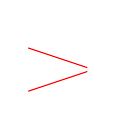
\begin{tikzpicture}
    \draw (-1,1) -- (-1,1);
    \begin{scope}[color=red]
      \draw (-1,0.75) -- (-0.25,0.5);
      \draw (-1,0.2) -- (-0.25,0.45);
    \end{scope}
  \end{tikzpicture}}

\begin{table}
  \begin{whole}
  \begin{tabular}{rrrclrrrr}

    &
    &
    &
    \multicolumn{2}{c}{$Mdn_A$} \\

    &
    \multicolumn{1}{c}{$N$} &
    \multicolumn{1}{c}{$Mdn$} &
    \multicolumn{2}{c}{$- Mdn_B$} &
    \multicolumn{1}{c}{$Rng$} &
    \multicolumn{1}{c}{$U$} &
    \multicolumn{1}{c}{$Z$} &
    \multicolumn{1}{c}{$p$} \\

    \cmidrule(lr){2-9}

    Experiement ($A$) &
    12 &
    5 &
    \multirow{2}{*}{\twoguides} &
    \multirow{2}{*}{1} &
    4 &
    \multirow{2}{*}{45} &
    \multirow{2}{*}{-1.353} &
    \multirow{2}{*}{0.089}\\

    Control ($B$) &
    11 &
    4 &
    &
    &
    3 \\

  \end{tabular}
  \caption[Up-to-date on Favorites' Activities, Between Groups]{%
    Up-to-date on favorites' activities comparison between
    experiment and control group for the posttest.
  }
  \label{table:uptodate.favorite.activities.between}
  \end{whole}
\end{table}

The results show that the median degree of acceptance to the statement
is higher for experiment respondents having used an activity stream than
control respondents with a placebo. This difference is however
not statistically significant.

We also tested if there was a change in acceptance within the respondent
groups from before they were given a treatment or placebo and after.
The results can be seen in
\tableref{uptodate.favorite.activities.within}.

\newcommand{\fourguides}{%
  \begin{tikzpicture}
    \draw (-1,1) -- (-1,1);
    \begin{scope}[color=red]
      \draw (-1,0.5) -- (-0.25,0.025);
      \draw (-1,-0.5) -- (-0.25,-0.025);
    \end{scope}
    \draw (-1,-1) -- (-1,-1);
  \end{tikzpicture}}

\begin{table}
  \begin{whole}
  \begin{tabular}{rrrrccclrrrr}

    &
    &
    &
    &
    \multicolumn{2}{c}{Post} &
    \multicolumn{2}{c}{$Mdn_A$} \\

    &
    &
    \multicolumn{1}{c}{$N$} &
    \multicolumn{1}{c}{$Mdn$} &
    \multicolumn{2}{c}{$-$ Pre} &
    \multicolumn{2}{c}{$- Mdn_B$} &
    \multicolumn{1}{c}{$Rng$} &
    \multicolumn{1}{c}{$T$} &
    \multicolumn{1}{c}{$Z$} &
    \multicolumn{1}{c}{$p$} \\

    \cmidrule(lr){3-12}

    \multirow{2}{*}{Experiment ($A$)} &
    Pre &
    14 &
    3 &
    \multirow{2}{*}{\twoguides} &
    \multirow{2}{*}{2} &
    \multirow{4}{*}{\fourguides} &
    \multirow{4}{*}{1} &
    4 &
    \multirow{2}{*}{10} &
    \multirow{2}{*}{-1.513} &
    \multirow{2}{*}{0.086}\\

    &
    Post &
    12 &
    5 &
    &
    &
    &
    &
    4 \\

    \multirow{2}{*}{Control ($B$)} &
    Pre &
    11 &
    3 &
    \multirow{2}{*}{\twoguides} &
    \multirow{2}{*}{1} &
    &
    &
    3 &
    \multirow{2}{*}{16} &
    \multirow{2}{*}{-0.787} &
    \multirow{2}{*}{0.258}\\

    &
    Post &
    11 &
    4 &
    &
    &
    &
    &
    3 \\

  \end{tabular}
  \caption[Up-to-date on Favorites' Activities, Within Groups]{%
    Up-to-date on favorites' activities  comparison between
    pretest and posttest within the experiment and control group.
  }
  \label{table:uptodate.favorite.activities.within}
  \end{whole}
\end{table}

The data shows that the median acceptance rate have rosen from the pretest to
the posttest for both experiment and control respondents. The acceptance of
the statemnent about how easy it is to keep up-to-date on favorites'
activities have rosen more for the respondents having used an activity stream
than those with a placebo. Neither of these increases of median values
are statistically significant.

\parabreak

While we observed increases in how easy respondents felt they could keep
up-to-date with favorites' activities when an activity stream was used none of
this data was statistically significant. Due to lack of evidence we can not
reject $H_0$.

\subsubsection{%
  Can social navigation trough activity streams help users keep
  up-to-date on favorites' specific activities on \urort{}?
}

Based on the statements:
\begin{items}
  \item It's easy to keep up-to-date on whether my favorites publishes
    new songs on \urort{}.
  \item It's easy to keep up-to-date on whether my favorites publishes
    new blog posts on \urort{}.
  \item It's easy to keep up-to-date on whether my favorites are
    performing at concerts.
  \item It's easy to keep up-to-date on the reactions other users at
    \urort{} have towards my favorite artists' songs.
\end{items}

we graded respondents answers as follows:

\begin{items}
  \item Fully disagree: 1
  \item Somewhat disagree: 2
  \item Neither agree nor disagree: 3
  \item Somewhat agree: 4
  \item Fully agree: 5
\end{items}

The $H_0$ stated that we would not see any positive change in how easy
respondents felt it was to keep up-to-date on favorites' specific activities
after introducing an activity steam. Our $H_A$ said that we
would indeed observe a change in how respondents rated this task.

First we compared how easy responents felt it was to keep up-to-date on
favorites' specific activities after they are given a treatment
or a placebo.
See
\tableref{uptodate.favorite.specific.activities.between} for the results.

\begin{table}
  \begin{whole}
  \begin{tabular}{rrrclrrrrl}

    &
    &
    &
    \multicolumn{2}{c}{$Mdn_A$} \\

    &
    \multicolumn{1}{c}{$N$} &
    \multicolumn{1}{c}{$Mdn$} &
    \multicolumn{2}{c}{$- Mdn_B$} &
    \multicolumn{1}{c}{$Rng$} &
    \multicolumn{1}{c}{$U$} &
    \multicolumn{1}{c}{$Z$} &
    \multicolumn{1}{c}{$p$} \\

    \cmidrule(lr){2-9}

    Experiment ($A$) &
    12 &
    5 &
    \multirow{2}{*}{\twoguides} &
    \multirow{2}{*}{1,0} &
    4 &
    \multirow{2}{*}{59} &
    \multirow{2}{*}{-0.479} &
    \multirow{2}{*}{0.340} &
    \multirow{2}{*}{Song}\\

    Control ($B$) &
    11 &
    4 &
    &
    &
    2 \\

    \cmidrule(lr){2-9}

    Experiment ($A$) &
    12 &
    4.5 &
    \multirow{2}{*}{\twoguides} &
    \multirow{2}{*}{1.5} &
    4 &
    \multirow{2}{*}{59} &
    \multirow{2}{*}{-0.460} &
    \multirow{2}{*}{0.289} &
    \multirow{2}{*}{Blog}\\

    Control ($B$) &
    11 &
    3 &
    &
    &
    2 \\

    \cmidrule(lr){2-9}

    Experiment ($A$) &
    12 &
    3.5 &
    \multirow{2}{*}{\twoguides} &
    \multirow{2}{*}{-0.5} &
    4 &
    \multirow{2}{*}{66} &
    \multirow{2}{*}{0.000} &
    \multirow{2}{*}{0.517} &
    \multirow{2}{*}{Concert}\\

    Control ($B$) &
    11 &
    4 &
    &
    &
    3 \\

    \cmidrule(lr){2-9}

    Experiment ($A$) &
    12 &
    3.5 &
    \multirow{2}{*}{\twoguides} &
    \multirow{2}{*}{0.5} &
    4 &
    \multirow{2}{*}{60} &
    \multirow{2}{*}{-0.385} &
    \multirow{2}{*}{0.372} &
    \multirow{2}{*}{Review}\\

    Control ($B$) &
    11 &
    3 &
    &
    &
    3 \\

  \end{tabular}
  \caption[Up-to-date on Favorites' Specific Activities, Between Groups]{%
    Up-to-date on favorites' specific activities comparison between
    experiment and control group for the posttest.
  }
  \label{table:uptodate.favorite.specific.activities.between}
  \end{whole}
\end{table}

The reported median degree of how easy it is to keep up-to-date
on new songs, blogs posts, and reviews is higher for those
which used an activity stream than those without. Respondents using
and activity stream reported a lower median value of how easy it was
to keep up-to-date on concerts compared to those without such treatment.
Neither the increases and decreases in the median degree from the
control group to the experiment group were stastically significant.

As for general activities we also tested whether respondents perception
of how easy it was to keep up-to-date on specific activities from
favorites had changed from before a treatment or placebo was given to after.
See 
\tableref{uptodate.favorite.specific.activities.within} for the results of the
in group comparisons.

\begin{table}
  \begin{whole}
  \begin{tabular}{rrrrccclrrrrl}

    &
    &
    &
    &
    \multicolumn{2}{c}{Post} &
    \multicolumn{2}{c}{$Mdn_A$} \\

    &
    &
    \multicolumn{1}{c}{$N$} &
    \multicolumn{1}{c}{$Mdn$} &
    \multicolumn{2}{c}{$-$ Pre} &
    \multicolumn{2}{c}{$- Mdn_B$} &
    \multicolumn{1}{c}{$Rng$} &
    \multicolumn{1}{c}{$T$} &
    \multicolumn{1}{c}{$Z$} &
    \multicolumn{1}{c}{$p$} \\

    \cmidrule(lr){3-12}

      \multirow{2}{*}{Experiment ($A$)} &
        Pre &
        14 &
        4 &
        \multirow{2}{*}{\twoguides} &
        \multirow{2}{*}{1} &
        \multirow{4}{*}{\fourguides} &
        \multirow{4}{*}{0} &
        4 &
        \multirow{2}{*}{8.0} &
        \multirow{2}{*}{-1.780} &
        \multirow{2}{*}{0.049} &
        \multirow{4}{*}{Song} \\

        &
        Post &
        12 &
        5 &
        &
        &
        &
        &
        4 \\

      \multirow{2}{*}{Control ($B$)} &
        Pre &
        11 &
        3 &
        \multirow{2}{*}{\twoguides} &
        \multirow{2}{*}{1} &
        &
        &
        3 &
        \multirow{2}{*}{4.0} &
        \multirow{2}{*}{-1.709} &
        \multirow{2}{*}{0.055} &
        \\

        &
        Post &
        11 &
        4 &
        &
        &
        &
        &
        2 \\

    \cmidrule(lr){2-12}

      \multirow{2}{*}{Experiment ($A$)} &
        Pre &
        14 &
        3 &
        \multirow{2}{*}{\twoguides} &
        \multirow{2}{*}{1.5} &
        \multirow{4}{*}{\fourguides} &
        \multirow{4}{*}{1.5} &
        3 &
        \multirow{2}{*}{9.5} &
        \multirow{2}{*}{-1.872} &
        \multirow{2}{*}{0.039} &
        \multirow{4}{*}{Blog} \\

        &
        Post &
        12 &
        4.5 &
        &
        &
        &
        &
        4 \\

      \multirow{2}{*}{Control ($B$)} &
        Pre &
        11 &
        3 &
        \multirow{2}{*}{\twoguides} &
        \multirow{2}{*}{0} &
        &
        &
        3 &
        \multirow{2}{*}{13.0} &
        \multirow{2}{*}{-1.150} &
        \multirow{2}{*}{0.166} &
        \\

        &
        Post &
        11 &
        3 &
        &
        &
        &
        &
        2 \\

    \cmidrule(lr){2-12}

      \multirow{2}{*}{Experiment ($A$)} &
        Pre &
        14 &
        3 &
        \multirow{2}{*}{\twoguides} &
        \multirow{2}{*}{0.5} &
        \multirow{4}{*}{\fourguides} &
        \multirow{4}{*}{-0.5} &
        3 &
        \multirow{2}{*}{7.5} &
        \multirow{2}{*}{-1.127} &
        \multirow{2}{*}{0.188} &
        \multirow{4}{*}{Concert} \\

        &
        Post &
        12 &
        3.5 &
        &
        &
        &
        &
        4 \\

      \multirow{2}{*}{Control ($B$)} &
        Pre &
        11 &
        3 &
        \multirow{2}{*}{\twoguides} &
        \multirow{2}{*}{1} &
        &
        &
        3 &
        \multirow{2}{*}{5.5} &
        \multirow{2}{*}{-1.063} &
        \multirow{2}{*}{0.203} &
        \\

        &
        Post &
        11 &
        4 &
        &
        &
        &
        &
        3 \\

    \cmidrule(lr){2-12}

      \multirow{2}{*}{Experiment ($A$)} &
        Pre &
        13 &
        3 &
        \multirow{2}{*}{\twoguides} &
        \multirow{2}{*}{0.5} &
        \multirow{4}{*}{\fourguides} &
        \multirow{4}{*}{1.5} &
        4 &
        \multirow{2}{*}{4.5} &
        \multirow{2}{*}{-1.298} &
        \multirow{2}{*}{0.125} &
        \multirow{4}{*}{Review} \\

        &
        Post &
        12 &
        3.5 &
        &
        &
        &
        &
        4 \\

      \multirow{2}{*}{Control ($B$)} &
        Pre &
        11 &
        4 &
        \multirow{2}{*}{\twoguides} &
        \multirow{2}{*}{-1} &
        &
        &
        3 &
        \multirow{2}{*}{9.5} &
        \multirow{2}{*}{-0.780} &
        \multirow{2}{*}{0.281} &
        \\

        &
        Post &
        11 &
        3 &
        &
        &
        &
        &
        3 \\

  \end{tabular}
  \caption[Up-to-date on Favorites' Specific Activities, Within Groups]{%
    Up-to-date on favorites's specific activities comparison between
    pretest and posttest within the experiment and control group.
  }
  \label{table:uptodate.favorite.specific.activities.within}
  \end{whole}
\end{table}

The within group data shows that experiment respondents and control
respondents find it easier to keep up-to-date on rencent songs
and concert performances after the treatment or placebo was given.
The increases are of the same order for both those which used an
activity stream and those without. Neither of the two groups increases
for concerts is statistically significant.
The experiment groups' increase is significant for songs while the control
groups' increase for songs is insignificant.
Note that the difference between $p$ values for the two groups related to
songs are marginal.

Respondents having used an activity stream saw an increase in median
response from \q{neither agree or disagree} to \q{fully agree} regarding
how easy it was to keep up-to-date on blog posts of favorites.
This difference is statistically significant.
The control group saw no such increase after they were given a placebo.

On the topic of how easy respondents could keep up-to-date on
reviews of favorites' songs the experiment group saw no change
after treatment while the control group saw a decrease after having used
a placebo. This decrease is not statistically significant.

\parabreak

None of the differences we found with regards to specific activities between
the experiment and control group for the posttest was significant.
We can't reject $H_0$ for any of the specific activities based on this
evidence. Well look at how $H_0$ stands based on the difference within groups
from before treatment and placebo were given to after for each specific
activity:

\begin{items}
  \iterm{Song:} We did find significant evidence
    of a an increase in ease of keeping up-to-date on songs for respondents
    which used an activity stream while those without had insignificant
    increases. The difference of significance were quite small so $H_0$
    stands unrejected for songs.
  \iterm{Blog:} The respondents which had used an activity list saw a
    significant increase in their median ranks of how easy it was
    to keep up-to-date on blogs. The respondents having used our placebo
    saw no such increase. Based on this evidence we reject $H_0$ in favor
    of $H_A$ for keeping up-to-date on blog posts.
  \iterm{Concert:} Both experiment and control groups saw
    statistically insignificant increases in their median degree of how easy
    the task was for concerts. $H_0$ therefore stands unrejected for concerts.
  \iterm{Review:} For reviews we noticed no significant increases or decreases
    of the median degree of how easy it was to keep up-to-date. 
    $H_0$ therefore stands unrejected for reviews.
\end{items}

\clearpage
\clearpage

\section{Discussion}

\subsection{Activity streams as a social navigation technique}

\subsection{Transparent prototyping with Greasemonkey}

During our development of a prototype application with Greasemonkey for
enhancing an established web page we got a feel for its pros and cons from a
development perspective.

\subsubsection{Requires no access to the established implementation}

\subsubsection{Requires little knowledge of the established implementation}

\subsubsection{Requires more work than altering the established
  implementation}

\subsubsection{Fragile when the established implementation is changed}
% Only happened once during a two month span on \urort{}. What was scary
% thought was that the changes made the user script on the client side
% obsolete. If this had happened under production usage when the user scripts
% was pushed to the clients we would be in a world of trouble. Changes on the
% server side platform can be handled more transparently.

\subsubsection{Less performant than the established implementation}

\parabreak

When we conducted a study of our prototype with real world users
we got valuable feedback on how well such a system works for the average user.

\subsubsection{Limited in browser selection}

\subsubsection{Difficulties with installing Greasemonkey}

\subsubsection{Difficulties with installing user-scripts}

\section{Generalizability and Validity}
